% ************ Capítulo 1 ************
%\renewcommand{\chaptername}{Capítulo}
\chapter{Introdução}
\label{cap:1}

\section{Enquadramento}
A reciclagem de residuos de velas ainda não é neste momento uma ativadade com grande expressão no mercado Português. Existem apenas algumas empresas atualamente a fazer a reciclagem deste tipo de residuos e as suas principais fontes de materia-prima são os cemitétios e locais de culto religioso, onde o uso de velas é uma pratica muito comum. Entre as entidades que operam neste setor podemos mencionar o Santuário de Fátima\cite{DesktakFatima}, o Centro Ambiental do Carvalho de Calvos\cite{SecundinoCunha2016} e a Natural Life\cite{NaturalLife}.

\section{Apresentação da empresa}
A Natural Life, Lda. é uma empresa fundada em 2013. Está sediada na rua de terramonte nº 781, Armazém C20, na Maia. Tendo como atividade a recolha e reciclagem de resíduos de velas, a Natural Life surge como uma empresa ecológica, inteiramente ligada a área Ambiental, mais concretamente à Reciclagem.\cite{NaturalLife}\\
A empresa cuida de todo o processo, desde a recolha da materia-prima nos cemiterios com as quais tem parceria, a separação do corpo de plastico, da tampa de metal e da cera até à fundição da cera. Em alguns casos a recolha do material é substituida por material recolhido por terceiros, mantendo-se o resto do processo.
O espaço físico da fabrica esta divido em duas partes: a primeira onde fica o armazem e onde é rececionado a materia-prima e um segundo espaço onde esta uma maquina que corta o corpo de plástico do círio, tendo apenas de o colaborador da frente abrir o corpo e seprar a cera do plastico. A alimentar esta maquina esta um operador que recebe o corpo do círio sem nenhum elemento metalico, tendo apenas que colocar o cirio devidamente alinhado. Alguns cirios, devido à sua forma, não podem ser colocadosFinita a separação a cera é enviada para o forno. Quando a cera termina de ser deretida é enformada e colocada num espaço de ar condicionado para arrefecer e solidificar. Normalmente este processo é feito ao fim do dia e durante a noite para poder aproveitar a baixa de temperatura ambeintal.

\begin{figure}[H] 
	\begin{center}
		% Requires \usepackage{graphicx}
		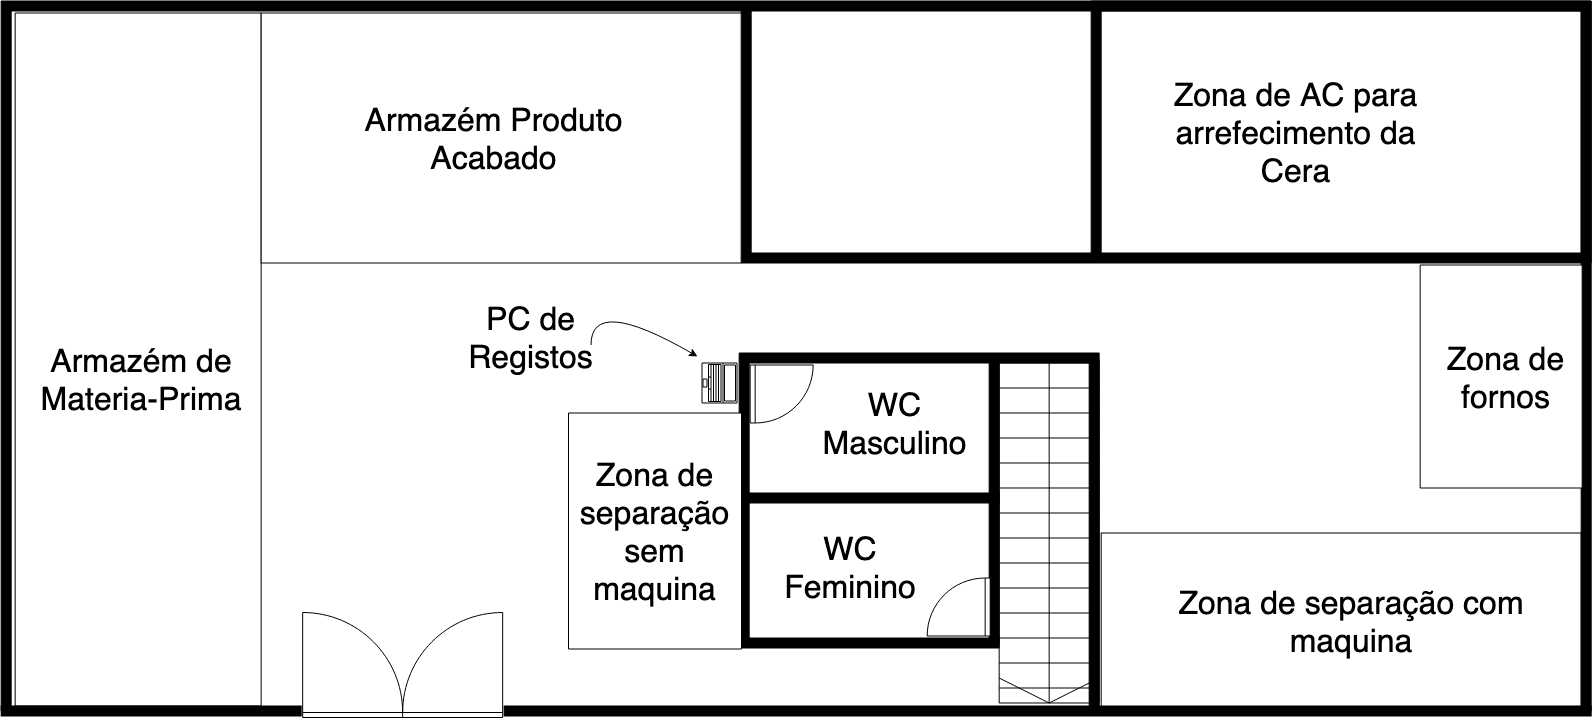
\includegraphics[width=\textwidth,keepaspectratio]{figuras/PlantaNaturalLife.png}
		\caption{Planta da fábrica}\label{fig:planta_naturallife} 
	\end{center}
\end{figure}

A recolha da informação era feito por meio de uma base de dados desenvolvida com o software Microsoft Access\label{sym:MS_ACCESS} com auxilio de alguns formulários embutidos na mesma. Aquilo que se previa ser uma solução temporária, acabou por se tornar definitiva pela simplicidade que a interface oferecia aos utilizadores, pela simples integração com outras aplicações Microsoft, como o Microsoft Excel\label{sym:MS_EXCEL} e Microsoft PowerBI\label{sym:MS_POWERBI}, e pela dificuldade de encontrar um sistema ERP\label{sym:ERP} comercial com as características da solução temporária, com um custo de aquisição que a empresa pudesse comportar e permitisse obter interfaces simplistas para os utilizadores que já se tinham acostumado com os formulários em Access.
No entanto a solução desenvolvida no Microsoft Access é bastante limitada no que toca a executar o mesmo ficheiro em dois computadores ao mesmo tempo, o que limitava as opções da administração nos seus planos expansão da fábrica ou até fazer gestão da própria empresa. Este constrangimento obriga os colaboradores a deslocar-se vários metros até ao único computador da fábrica, onde a base de dados estava, para aí fazerem registos. Por fim esta base de dados não suporta níveis de acesso, o que quer dizer que qualquer pessoa com acesso ao computador poderá não só ver todos os registos da empresa como modificá-los ou até mesmo apagá-los.\\
Assim, pretende-se com este projeto de estágio a implementação de um novo sistema de recolha e consulta de informação, desenvolvido pelo aluno e consequente migração dos dados anteriormente registados.
\newpage



\section{Objetivos}
Implementar um sistema de informação (SI\label{sym:SI}) para efetuar o registo do ponto dos colaboradores, recolhas, produções, acabamento e saída do produto acabado. Esta solução teria de possuir duas areas distintas, a primeira destinada ao uso na fábrica e a segunda destinadaao uso pela adminstração.

%%%%%%%%%%%%%%%%%%%%%%%%%%%%%%%% Ainda tem de ser feiro %%%%%%%%%%%%%%%%%%%%%%%%%%%%%%%%%%
\section{Calendarização}
No Diagrama de Gantt a seguir é descrito as fases do projeto e a sua respetiva duração.

\begin{figure}[htbp] 
    \begin{center}
    % Requires \usepackage{graphicx}
    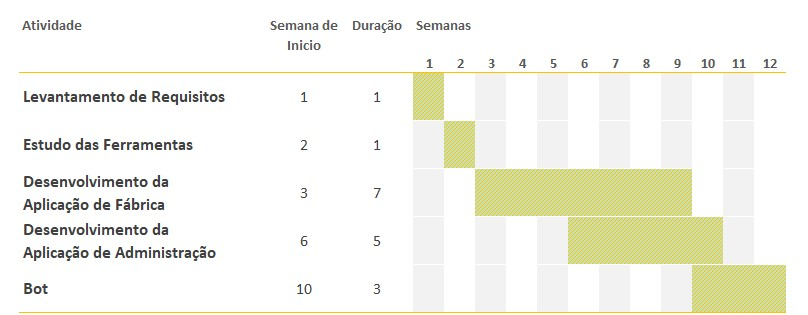
\includegraphics[width=\textwidth,keepaspectratio]{figuras/DiagramaGant.jpg}
    \caption{Gantt chart com o plano de trabalhos de PROES\label{sym:PROES}}\label{fig:gantt chart} 
    \end{center}
\end{figure}

\section{Organização do relatório}
No Capítulo 1 é feito o enquadramento do projeto dando uma visão alto nível do projeto. No capítulo 2, é apresentado o estado da arte. É neste capitulo que são descritas as diferentes opções para a realização do projeto e onde são descritas as escolhas feitas e o seu motivo. No capítulo 3 é apresentada a lista de requisitos e do projeto, bem como o processo para a sua obtenção. O capítulo 4, destina-se à descrição do desenvolvimento e implementação do projeto, apresentando em detalhes as características do trabalho desenvolvido.
Assim, no capítulo 5, são descritos os resultados da implementação e o \textit{feedback} geral recebido pela administração e pelos colaboradores da empresa. No último capítulo, o 6º, são apresentadas as conclusões do projeto, incluindo nestas a opinião crítica do estudante face ao trabalho desenvolvido.
